\chapter{Algorithm}
\label{ch:algorithm}

In this chapter the algorithm is discussed, presenting how the objects are recognized, and how the symbolic predicates are obtained. 

\section{Object Localization} 
For the planner, to know how to move the object, is fundamental knowing the objects on the scenario, therefore they need to be detected. More correctly, they need to be segmented since the algorithm is dealing with unknown objects, it is not going to recognize an objects as a particular one, but it segments the objects. 

This stage is composed on two steps:
\begin{enumerate}
\item Detecting the table top objects
\item Segmenting the table top objects
\end{enumerate}
The depth sensor is recording a depth map of a table, the algorithm has therefore to detect first the table, and so the objects that stands on top of it, and then segmenting them. We don't want to segment the entire image, if so, the table will be segmented as an object and the floor as well.

\subsection{Tabletop Object Detection} 
The strategy for the tabletop object detection phase is composed of 3 different steps:
\begin{enumerate}
\item \textbf{Table plane estimation} (by RANSAC): the points of the table are detected estimating first a plane in the point cloud, all the points which belong to such a plane are the points of the table. 
\item \textbf{2D Convex Hull of the table}: having the points of the table a 2D convex hull is computed in order to get a 2D shape containing those points.
\item \textbf{Polygonal prism projection}: all the points are projected on the table plane previously estimated and all the points which projections belong to the 2D convex hull are considered to be points of tabletop objects. 
\end{enumerate}

\begin{figure}[htp]
\centering
\begin{subfigure}[t]{0.32\textwidth}
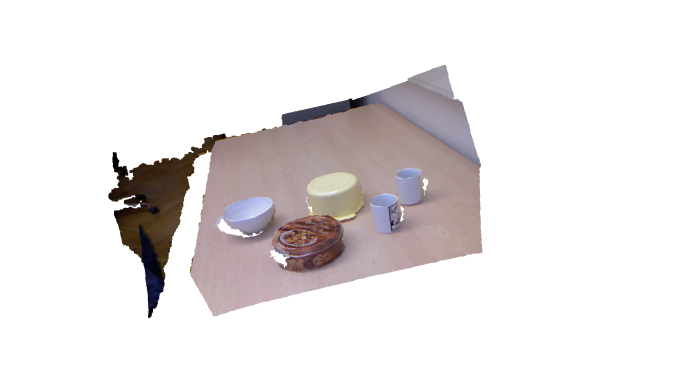
\includegraphics[width = 1.1\textwidth]{Img/ObjectSegmentation/pcl.png}
\caption{Input Point Cloud}\label{img:obj_pointcloud}
\end{subfigure}
\begin{subfigure}[t]{0.32\textwidth}
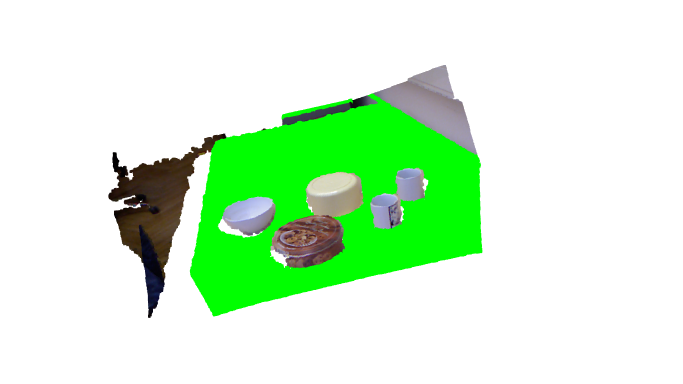
\includegraphics[width = 1.1\textwidth]{Img/ObjectSegmentation/ransac.png}
\caption{RANSAC plane estimation}\label{img:obj_ransac}
\end{subfigure}
\begin{subfigure}[t]{0.32\textwidth}
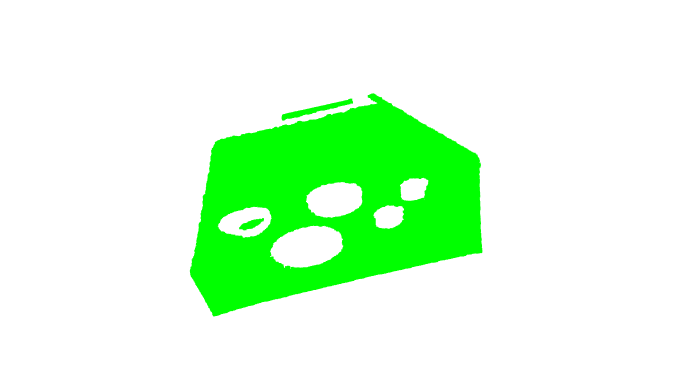
\includegraphics[width = 1.1\textwidth]{Img/ObjectSegmentation/plane.png}
\caption{Table plane}\label{img:obj_plane}
\end{subfigure}
\begin{subfigure}[t]{0.32\textwidth}
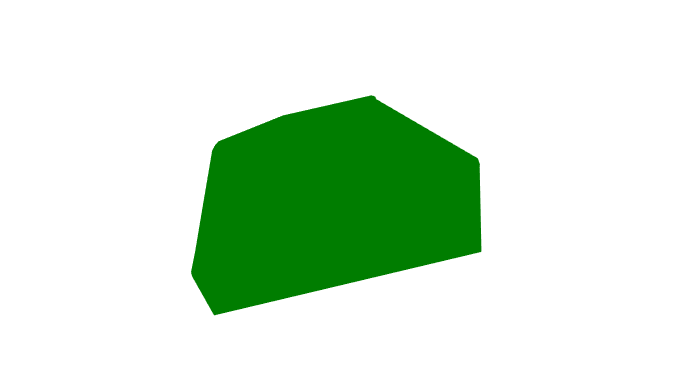
\includegraphics[width = 1.1\textwidth]{Img/ObjectSegmentation/convex_hull.png}
\caption{Convex Hull}\label{img:obj_conex_hull}
\end{subfigure}
\begin{subfigure}[t]{0.32\textwidth}
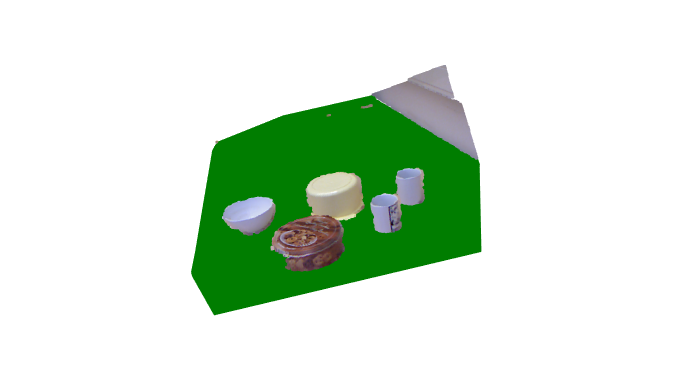
\includegraphics[width = 1.1\textwidth]{Img/ObjectSegmentation/convex_hull_full.png}
\caption{Convex hull in the point cloud}\label{img:obj_convex_hull_full}
\end{subfigure}
\begin{subfigure}[t]{0.32\textwidth}
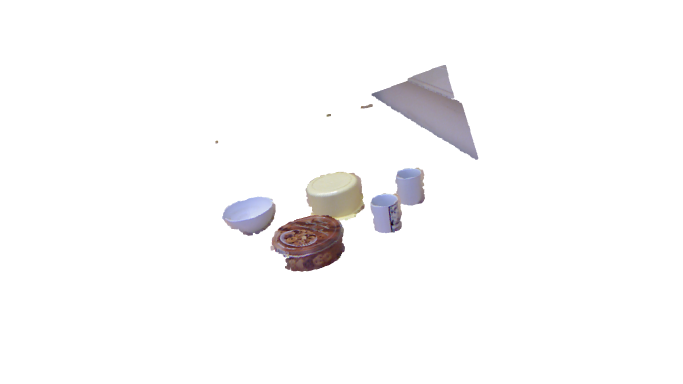
\includegraphics[width = 1.1\textwidth]{Img/ObjectSegmentation/tabletop_objects.png}
\caption{Tabletop objects}\label{img:obj_tabletop_objects_results}
\end{subfigure}
\caption{\textbf{Object Segmentation:} Given the point cloud (\subref{img:obj_pointcloud}), the estimated table's plane is obtained (\subref{img:obj_ransac} and \subref{img:obj_plane}), its convex hull is extracted (\subref{img:obj_conex_hull} and \subref{img:obj_convex_hull_full}), and the tabletop objects are obtained by a polygonal prism projection (\subref{img:obj_tabletop_objects_results}).}
\label{img:obj_tabletop_objects}
\end{figure}

The steps of this tabletop object detection algorithm are described in Figure \ref{img:obj_tabletop_objects}   for the point cloud in Figure \ref{img:obj_pointcloud}.

\subsection{Object Segmentation}
\label{sec:obj_seg}
Once the objects on the table are detected the following phase is to segment them in order to get a point cloud per object.

\subsubsection{Supervoxel}

For their segmentation the supervoxel concept is used. A supervoxel is a group of voxels that share similar characteristics. 
%and it is equivalent to the superpixel concept for the voxel case. Superpixel is a widely used preprocessing step in segmentation
%algorithms  which allows to reduce the number of regions
%that must be considered later by more computationally
%expensive algorithms, with a minimal loss of information. 
%The supervoxel concept is the extension of the superpixel method to the point clouds. A voxel represents a single sample on a regularly spaced, three-dimensional grid. A supervoxel 

In this work the supervoxels are computed with the Voxel Cloud Connectivy Segmentation (\texttt{VCCS}) algorithm \cite{Papon13CVPR}, which was proposed in 2014 and gives good improvements with respect to previous state of the art methods, and still it is able to be used in online applications. 

The algorithm works in 4 main steps:
\begin{itemize}
\item Voxelizing the point cloud
\item Creating an adjacency graph for the voxel-cloud 
\item Creating seeds for the initial supervoxels centres
\item Each seed is described by $39$ features that describe spatial coordinates, colors and local surface model properties. Then a distance metric based on  these features is defined. 
\item Clustering the voxels into supervoxles iteratively by means of the distance metric, the adjacency graph, and the search volume of the supervoxel. 
\item Once the search of all supervoxel adjacency graphs has been concluded, the centres of each supervoxel is updated by taking the mean of all its constituents. 
\end{itemize} 

\subsubsection{Local Convex Connected Patches Segmentation}
\label{sec:LCCP}
Once the supervoxels of the objects are computed, they can be clustered in order to segment the objects. Papon et al. also proposed a segmentation algorithm based on their supervoxel technique, called \textit{Local Convex Connected Patches Segmentation} (\texttt{LCCP}) \citep{LCCP}. This algorithm permits to segment objects by clustering together adjacent convex supervoxels.  The algorithm is quite simple but very good for segmentation of objects that have convex shapes, in Figure \ref{img:LCCP_structure} the algorithm is briefly described. 

\begin{figure}[h]
\centering
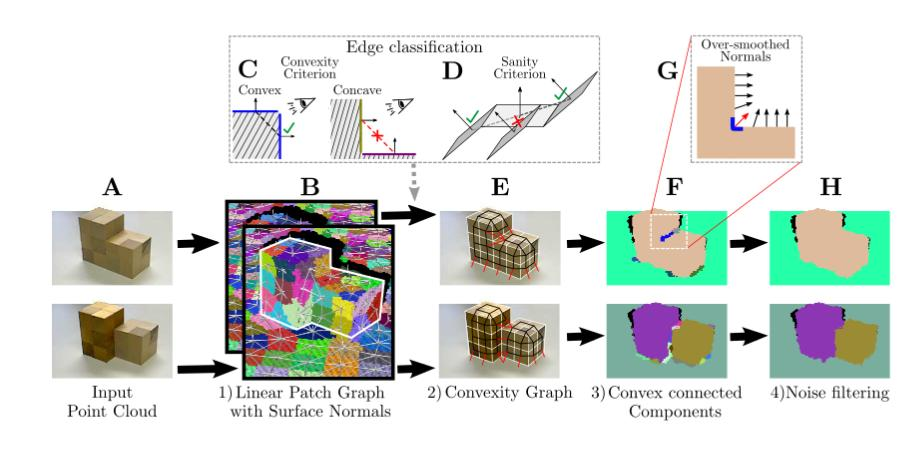
\includegraphics[width=\textwidth]{Img/ObjectSegmentation/lccp_structure.jpg}
\caption{\texttt{LCCP} algorithm's structure. Reproduced from \citep{LCCP}}
\label{img:LCCP_structure}
\end{figure}

It clusters all the adjacent convex supervoxels (patches) using two criterion:
\begin{itemize}
\item Extended criterion: to consider two adjacent patches convex, both must have a connection to a patch which is convex with respect both patches
\item Sanity Criterion: check if the adjacent patches which can be considered as convex present geometric discontinuities (see point D of Figure \ref{img:LCCP_structure}), in this case they are not considered as valid to form a cluster.
\end{itemize}
Then, due to the smoothed normals that could appear in some edges of the objects (point G Figure \ref{img:LCCP_structure}), the algorithm merges the clusters that are composed of few supervoxels to the biggest adjacent cluster. 

By tuning properly the parameters of the segmentation algorithm the objects can be correctly segmented obtaining for one of them a point cloud. 

\mbox{\textbf{ADD EXAMPLE IMAGES}}

\section{Predicates Computations}
Once the objects are segmented, we will have one point cloud per object, next we have to translate the scenario composition into symbolic predicates. 

In Chapter \ref{ch:task_planner}  the predicates that are used are described, in this section their computation is presented. 

Before going in detail on their computation some general concepts are first presented. 

\subsection{Tools}
\begin{itemize}
\item collison detection
\item pca
\item table projection - convex hulls
\end{itemize}
To understand if an object imped a certain action, such as the pushing along a direction, we have to check if along the desired trajectory the pushed object will collide with a certain one. The collision detection is therefore a crucial step for the predicates computation. For the collision checking the Flexible Collision Library (FCL) \citep{pan2012fcl} has been used. This library allows to define the collision problem in a simpler manner than other more famous collision libraries such as \textit{Bullet} \citep{Bullet}, and it can work with different objects shapes such as box, spheres, cone, convex, mesh and octree. 
The main library used in this work is the Point Cloud Library (PCL) \citep{PCL}, which allows some methods to create an object shape from a point cloud. The mesh shape has been thought to use since it can be easily obtained by using the \textit{convex hull} algorithm. 

Explain convex hull.

The PCL convex hull algorithm returns the convex hull as a triangular mesh, which can be used by the FCL for the collision detection. 

The pose of the Kinect camera is above the table pointing forward it. In such a pose the Kinect is only able to see mainly the top side of the objects, and not their sides. 
--- discussed the convex hull relating into to the neccesity for the collision detection.

\subsection{Predicate: \texttt{block\_grasp}}
\subsection{Predicate: \texttt{on}}
\subsection{Predicate: \texttt{block\_dir$_i$}}
